\documentclass{article}
\usepackage[utf8]{inputenc}

\usepackage{graphicx}
\usepackage{float}
\usepackage{subcaption}
\usepackage{changepage}

\begin{document}

\title{Optimizing Television Content for Video on Demand, Algorithmically Detecting Opening/Closing Credits, Recaps and Bumpers in TV Shows\'{} Video Files}
\author{Master Thesis\\ \\ Niels ten Boom  \\ s4767314}

\date{\vspace{-3ex}}

\maketitle
\newpage

\tableofcontents
\newpage

\section{Introduction}
Viewing rates for TV are dropping gradually while the user counts of streaming services such as Netflix and Videoland are growing year over year. This shift from TV to Video on Demand introduces new problems for broadcasters (in this case RTL), as they now have to support a hybrid form of traditional broadcasting and Video On Demand (VOD). RTL does this by putting their content on Videoland after it has aired on TV. 

Video content is optimized for just one form, and currently that is TV. This means that the video content contains recaps, opening credits, bumpers (to ease a viewer into commercials) and closing credits. A viewer watching this content back-to-back may find it preferable to be able to skip these recurring segments to improve their viewing experience. Providing this functionality to users, requires metadata on where the skippable segments occur in the videos. For a large percentage of their content, such metadata has not been retained. Videoland currently hosts over 1000 different titles consisting of multiple seasons and episodes and this selection is prone to change. An automated solution that can detect these segments in videos would be very useful to solve that problem and transform the video content into a format suited for VOD. In this thesis we will explore the best methods for such an automated solution. 
% Definities van series?

There is little margin for error with this solution. The accuracy of the end result should be sufficiently high enough for it to be trusted to label all of the content automatically. If that is not the case then it needs double checking by a human. Because if a part of the video gets mislabeled, a user may skip over actual content. It is critical to RTL that this does not happen.

This research presents my findings on detecting recaps, opening credits, bumpers and closing credits given the video files from a TV-show. Because this being looked at from a business perspective, the solution should also be cost effective, meaning it should be efficient. The research question then reads:
\newline
\begin{adjustwidth}{0.3in}{0.3in}
\textit{\textbf{To what extent is it possible to accurately detect recaps, opening credits, bumpers and closing credits in video files and what are the most efficient methods? \newline}}
\end{adjustwidth}
This thesis aims to answer aforementioned research question. The rest of this section will be used to define the different type of video classes which this research is focused on. Section \ref{relatedwork} explains all of the related work. In section \ref{data} the data is presented. Section \ref{methodology} expands on the methodology and then the produced results are presented in section \ref{results}. Lastly, the results are discussed in section \ref{discussion}.

\subsection{Segment classes}
In this section we will give a background on the different types of segments to be detected.

\subsubsection{Closing Credits}
The closing credits at the end of a video contain a lot of scrolling text most of the time and there is little variation between the frames. In these texts everybody related to the production of the video is mentioned. In general the frames all have a black background with white text. But backgrounds can also vary as can be seen in figure \ref{fig:closingcredits}, therefore a solution that simply detects black and white would not suffice.

\begin{figure}[H]
  \centering
  \begin{subfigure}[b]{0.4\textwidth}
    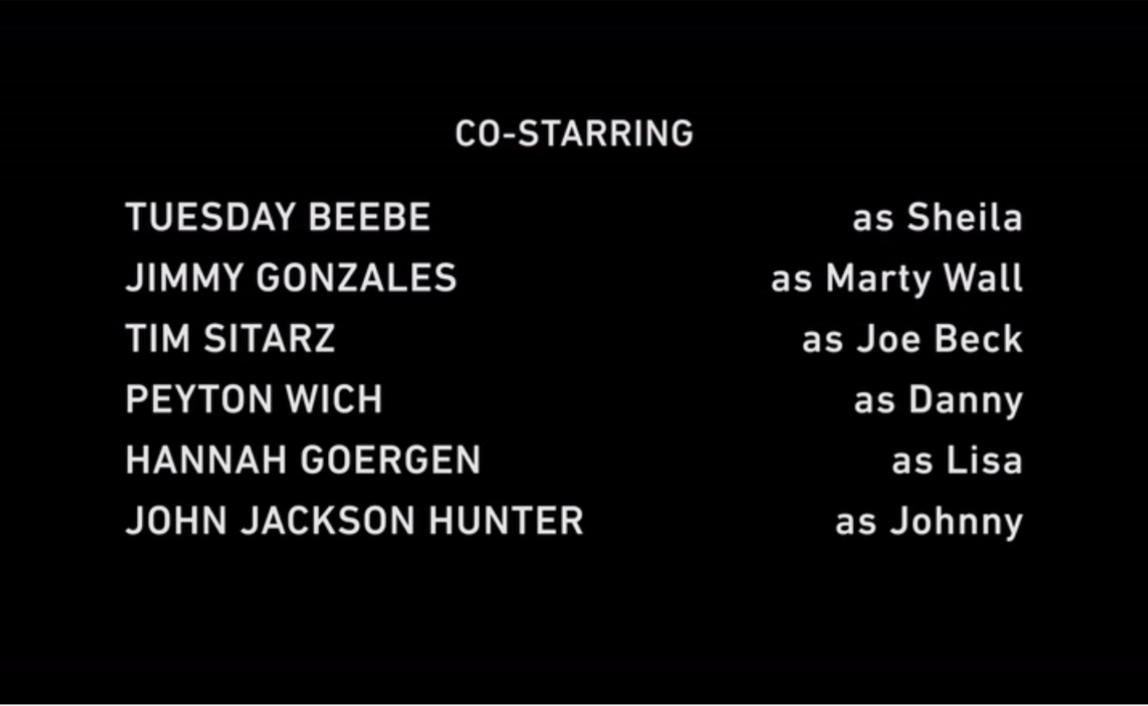
\includegraphics[width=\textwidth]{images/screencreditslarge.png}
  \end{subfigure}
  \begin{subfigure}[b]{0.4\textwidth}
    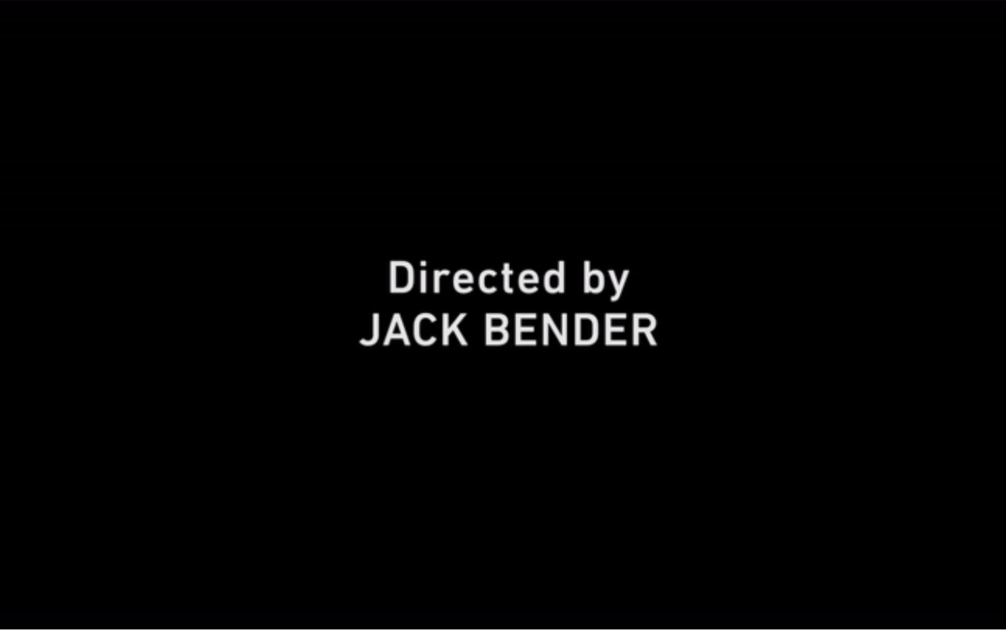
\includegraphics[width=\textwidth]{images/screencreditslarge2.png}
  \end{subfigure}
\begin{subfigure}[b]{0.4\textwidth}
	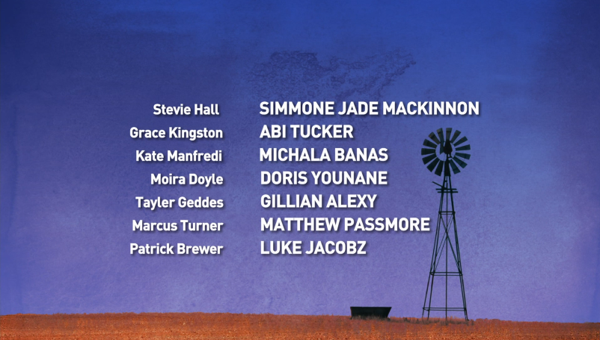
\includegraphics[width=\textwidth]{images/diffcredits.png}
\end{subfigure}
\begin{subfigure}[b]{0.4\textwidth}
	
\includegraphics[width=\textwidth]{images/diffcredits2.png}
\end{subfigure}
  \caption{Examples of varying types of closing credits}
  \label{fig:closingcredits}
\end{figure}

\subsubsection{Opening credits}
The opening credits of a TV-show are generally the same for at least all of the episodes in the same season. It opens the show with a theme song, presenting the most important actors at the start. If the sequence were known then it would be a rather simple problem to solve, by matching this sequence with all of the videos to locate the opening credits. The difficult part here is that they start somewhere at the start of a video, never right at the start. There is also no prior knowledge on how the opening credits of a show look like and they change every season.

\subsubsection{Recaps}
A television show may contain recaps before the opening credits. If this is the case, then a binge watcher ideally wants to skip this part together with the opening credits. Not all material preceeding the opening credits is a recap though, sometimes it is original content. Classifying whether the video part before the opening credits consists of recaps is important for a fully automated solution.

\subsubsection{Bumpers}
The bumper is a part of the video that eases a viewer into the upcoming commercial (see figure \ref{examplebumper}). Most of the times it has a voice over and text on screen saying: 'Next' (or the dutch translation of 'next') and some footage of what is to be expected after the commercial break is shown.

\begin{figure}[H]
    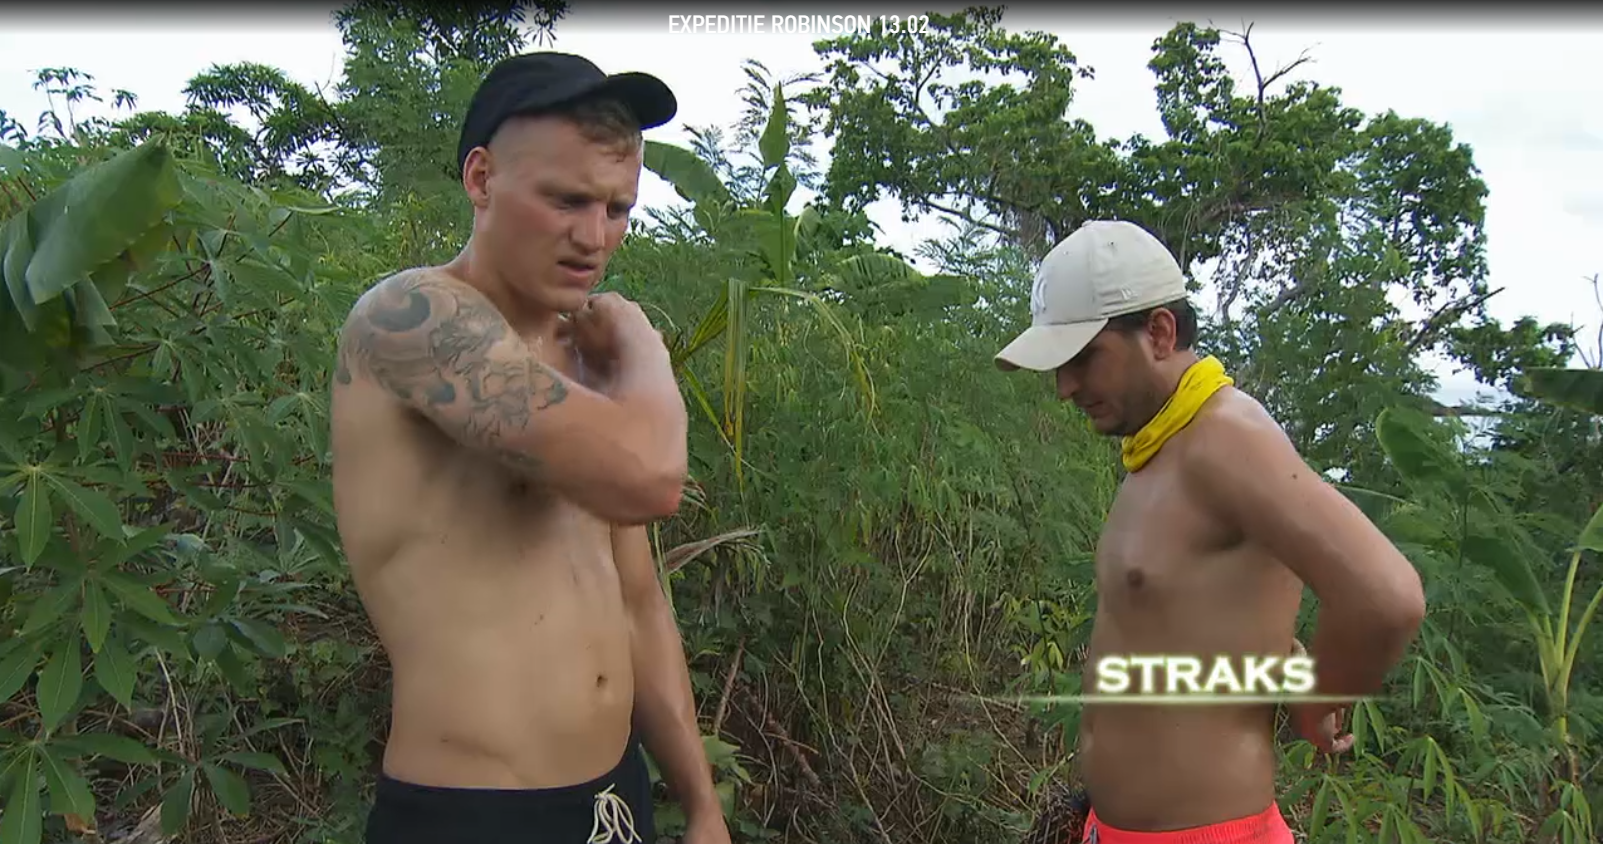
\includegraphics[width=7.5cm]{images/straks.png}
    \centering
    \caption{Example 'Next' bumper of the dutch television show Expeditie Robinson.}
    \label{examplebumper}
\end{figure}

\subsection{Definitions and Techniques}
This section will be used to elaborate on some topics mentioned in this thesis.

We define a season with multiple episodes of a TV-show as T.
\[T = \{E_1, E_2, \dots, E_x\}\]
An episode within a season is defined as a set of frames.
\[E = \{f_1, f_2, \dots, f_x\}\]


\subsubsection{Color Histograms}
A color histogram is a representation of the distribution of colors in an image. Color histograms are a flexible and low dimensional way of representing images. A color histogram can be computed by counting the number of pixels in a certain color range, the size of this range is variable, called the bin size. The higher the bin size, the lower the dimensions of the resulting histogram. See figure \ref{fig:colorhistogram} for an example color histogram where the bin size is 1, so each color is counted. 

\begin{figure}[H]
	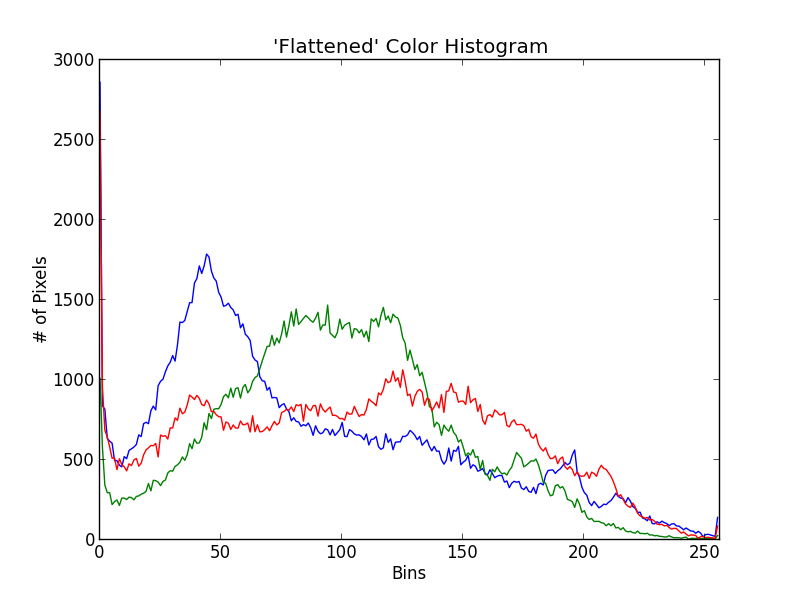
\includegraphics[width=8cm]{images/colorhistogram.png}
	\centering
	\caption{Color histograms with binsize n=1.}
	\label{fig:colorhistogram}
\end{figure}

Color histograms are going to be used to compute image similarity to match similar frames later in this thesis.

\subsubsection{Shot Change Detection}

Shot detection is a technique that can be used on videos to determine shot boundaries, see figure \ref{shotchange} for an example of such a shot change. 

\begin{figure}[H]
	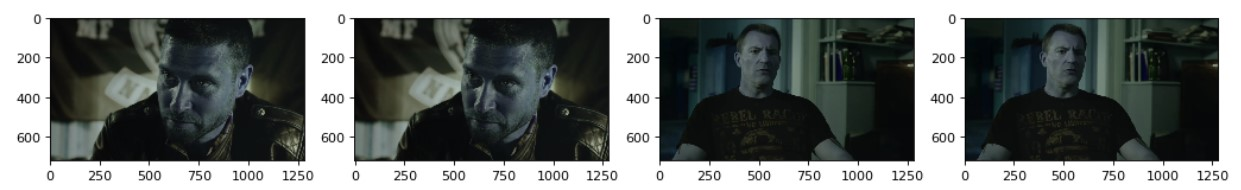
\includegraphics[width=12cm]{images/shotchange.jpg}
	\centering
	\caption{Example of a shot change.}
	\label{shotchange}
\end{figure}

Shot detection is going to be used and thus will we expand on it. A lot of research has been done related to shot detection \cite{lienhart1998comparison} and many techniques have been proposed. 

This thesis used a method that looks at the shift in mean color in HSV space \cite{shao2015shot}, see figure \ref{hsvspace} for a visual depiction of HSV color space. HSV (Hue, Saturation, Value) color space is a more intuitive color mixing model compared to RGB (Red, Green, Blue) color space. Because one can change a value in either of the three values in HSV and expect what the new color is going to look like. This is almost impossible for RGB because for this same color change to happen, you need to change all three red, green and blue values to result in the same color space.

\begin{figure}[H]
	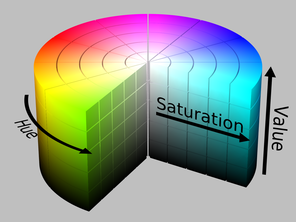
\includegraphics[width=5cm]{images/hsv.png}
	\centering
	\caption{The HSV color space.}
	\label{hsvspace}
\end{figure}

The shot boundaries are classified by calculating the difference in hue, saturation and value for each frame and then from this the mean is calculated. If the mean is higher than a threshold T, then a shot boundary is marked.

\section{Related Work} \label{relatedwork}

No prior work exists that explores a solution for the problem previously described (automatic labeling of segments).  A lot of related work exists that focuses on commercial or repeated sequence detection in large broadcast streams. These detection methods can be divided into three groups: fingerprint, feature-based and unsupervised methods. 

%fingerprint
With fingerprint methods the work sets up a database of fingerprints of known commercials or repeated sequences to detect these in a broadcast stream. Lienhart et al.\ \cite{lienhart1997detection} propose a method based on features to roughly localize advertisements in a stream and then construct a fingerprint database based on color coherence vectors. Gauch et al.\ \cite{gauch2006finding} propose a method based on the color moments in a stream. Covell et al.\ \cite{covell2006advertisement} implement a fingerprinting method based on audio with visual verification after a proposed match. The disadvantage of these fingerprinting methods is the setting up and maintenance of such a fingerprint database. 

%fingerprint methodes geven vaak ook methode voor repeated sequence detection maar met onvoldoende precisie

%feature based
The feature-based methods detect commercials based on extracted video features.  by looking at the changing color schemes to locate advertisements in a stream and then . Wang et al.\ \cite{wang2008multimodal} fuse the results of audio scene changes and textual content similarity between shots to segment programs including commercials.

%clustering
With the unsupervised methods the authors typically do a dimensionality reduction operation and then try to find repeated sequences or commercials with clustering methods. Herley et al.\ \cite{herley2006argos} convert the stream with a Discrete Cosine Transform (DCT) for dimensionality reduction and then propose an extensive probability framework to detect repeated sequences. Benezeth et al.\ \cite{benezeth2010unsupervised} use the Electronic Programme Guide (EPG) in addition to the dimensionality reduction to detect program boundaries.

%vergelijkbare dingen
Abduraman et al.\ \cite{abduraman2011unsupervised} propose a system to detect repeated sequences in streams by performing a DCT operation on all of the frames in the stream and then use a micro clustering technique to detect repeated sequences. They were also able to link the trailers to their respective programs that occur at a later point in the stream.

All of the previously mentioned works in this section never cover the specific topic of segmenting credits, recaps and bumpers. The methods yielded high accuracies in the range of 90\% - 95\% precision. This work aims for higher accuracies and thus will not be replicating most of the previously mentioned methodologies, however from the aforementioned papers we conclude that a large dimensionality reduction step will be necessary to process a large dataset of videos.

\iffalse
%oude paper OCR op video
\cite{li2000automatic} %TODO

%fingerprints
\cite{lienhart1997detection} %commercial detection met fingerprints
\cite{covell2006advertisement} %commercial detection fingerprints

%features
\cite{gauch2006finding} %commercial detection features
\cite{wang2008multimodal} %doen programma segmentatie

%clustering
\cite{herley2006argos} %argos paper gebruikt audio en heel veel probability
\cite{berrani2008non} %micro clustering repeated sequence detection

\cite{benezeth2010unsupervised} %enige paper die iets vergelijkbaars doet, maar op basis van stream en programmagids, veel nuttige references
\cite{ibrahim2011tv} %andere vergelijkbare paper, op advertenties en met grote stream
\cite{abduraman2011unsupervised} %Ook hele vergelijkbare paper, werken ook weer met DCT en KVD maar recall en precision round 0.95
\fi


\cite{zheng2018sift} Paper die alles omvat wbv image retrieval technieken.

\section{Data} \label{data}

The dataset contains 81 video files originating from 18 differing seasons of tv-shows. See the appendix for a full breakdown of the data. Originally these files were in .mxf full broadcast format, this meant each file being 25GB on average. All the files were converted to 1920p .mp4 files, resulting in each file being 1 GB on average.

For each file the start and end timestamps for the recaps, opening credits and closing credits were annotated in the HH:MM:SS format in a CSV file, so that it could be loaded effectively.

These files were then manually viewed and all the relevant segments were annotated. 

\section{Methodology} \label{methodology}

\subsection{Closing Credits}
Because the closing credits consist of mostly text, the first approach tried utilized text detection. The hypothesis of this approach was that when in a large video sequence for each analyzed frame text is found, then this sequence is the closing credits sequence.

Text detection was implemented by importing the open source OCR Tesseract package \cite{tesseract} in Python. Then the last 1/8 part of each video was analyzed by running text detection on multiples of the 24th frame. This was done because the videos were generally 24 frames per second and OCR is a costly computation. The hypothesis here was that by looking at one frame every second, the closing credits sequence could still be detected. The largest group of frames in sequence where Tesseract detected text in was classified as the closing credits.

This approach proved to be successful as can be seen in section \ref{resultsclosingcredits}. However sometimes the OCR would detect text in quite clearly textless images, sometimes this resulted in false classification of closing cred  its while the particular video did not contain any closing credits at all. Because of this, another detection step was introduced. An image classifier was trained to classify whether an image belongs to closing credits or to the rest of the video. The classifier was trained on 416 images of closing credits and 1062 images of other parts of the videos. These images were randomly extracted from the video data set. This classifier got a 100\% accuracy on a held out validation set of 245 images. The classifier was then used to verify that the detected start frame of the video really are closing credits. If the start frame was classified as non-credits and the total detected sequence was less than 5 seconds long. The video would be classified as not having any closing credits.

\subsection{Opening Credits}
We classified opening credits segments by converting frames to color histograms and then inspect the similarity matrices of videos. This is under the assumption that the opening credits are equal.

First, a color histogram for every frame is generated for every other x frames where $x \in \{3,6,12\}$. We do not compute a color histogram for every frame, the hypothesis for doing this is that it results in much faster processing times without losing accuracy, considering that increasing a similarity matrix its size increases the processing time quadratically. This results in a set of histograms H: 

\[H = \{h_1, h_2, \dots, h_x\}\]. 

Then we take $H_2$ and $H_x$ and compute the similarity matrix M, with the similarity defined as:

\[S({a, b}) = \sum_{i = 1}^{n} |a_i - b_i| \]

And from this similarity matrix we classify the part of a diagonal with the highest successive similarity as the opening credits. See figure \ref{simmatrix} for an example of such a diagonal with high similarity.

\begin{figure}[H]
	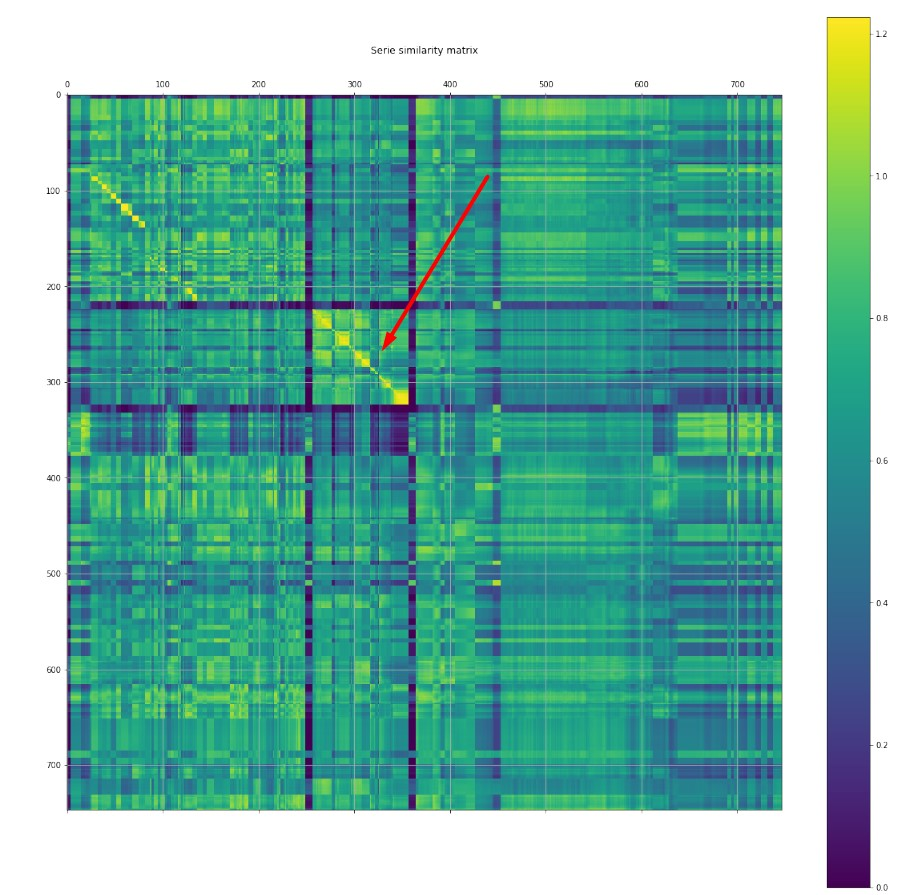
\includegraphics[width=10cm]{images/simmatrixarrow.jpg}
	\centering
	\caption{Plot of the similarity matrix of similarities between the color histograms of two episodes. The red arrow marks the location of the opening credits.}
	\label{simmatrix}
\end{figure}


\subsection{Recaps}
Early experimental results indicated that a solution based on recursively looking for similar frames in earlier episodes would not yield good results. We found that a feature based method to classify the segment before the opening credits as either recaps or non-recaps is an accurate method. 

The features are: Average shot length, presence of continuous sound, ratio of the length relative to the full episode.

\begin{figure}[H]
	\centering
	\begin{subfigure}[b]{0.4\textwidth}
		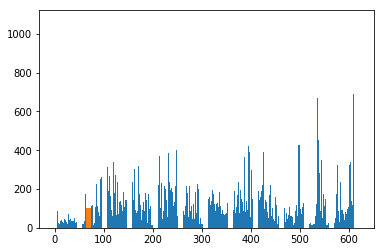
\includegraphics[width=\textwidth]{images/shotlengths_recaps_true.png}
	\end{subfigure}
	\begin{subfigure}[b]{0.4\textwidth}
		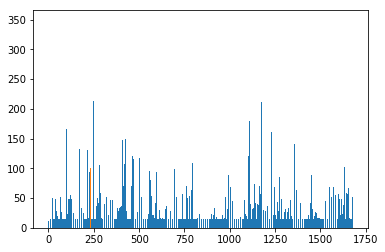
\includegraphics[width=\textwidth]{images/shotlengths_recaps_false.png}
	\end{subfigure}
	\caption{Bar plots of the shot lengths in frames. On the left is an episode with recaps. The episode on the right does not contain recaps. The bar in the other color marks the start of the opening credits.}
	\label{fig:closingcredits}
\end{figure}

\begin{figure}[H]
	\centering
	\begin{subfigure}[b]{0.4\textwidth}
		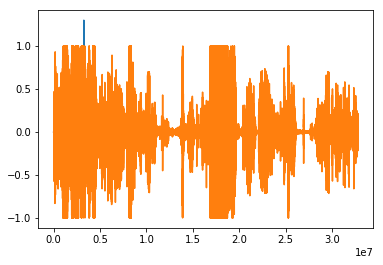
\includegraphics[width=\textwidth]{images/audio_recaps_true.png}
	\end{subfigure}
	\begin{subfigure}[b]{0.4\textwidth}
		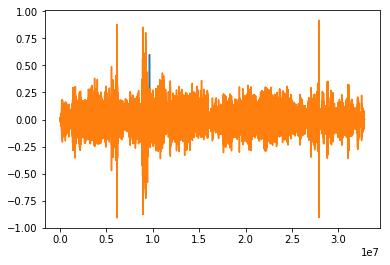
\includegraphics[width=\textwidth]{images/audio_recaps_false.png}
	\end{subfigure}
	\caption{Plots of the audio. On the left is an episode with recaps. The episode on the right does not contain recaps. The bar in the other color marks the start of the opening credits.}
	\label{fig:closingcredits}
\end{figure}

\subsection{Bumpers}

\section{Results} \label{results}

\subsection{Closing Credits}\label{resultsclosingcredits}
\subsection{Opening Credits}\label{resultsopeningcredits}
\subsection{Recaps}\label{resultsrecaps}
\subsection{Bumpers}\label{resultsbumpers}

\section{Discussion} \label{discussion}

\bibliographystyle{ieeetr}
\bibliography{references}

\end{document}
